\documentclass[final, hyperref={pdfpagelabels=false}]{beamer}
\mode<presentation>
\usetheme{UCLA}
\setbeamertemplate{caption}[numbered]

\usepackage{amsmath, amsthm, amssymb, latexsym}
\usepackage[english]{babel}
\usepackage[latin1]{inputenc}
\usepackage[%
  orientation=landscape,
  size=custom,
  width=160,  % cm
  height=100,  % cm
  scale=2,
  debug]{beamerposter}
\usepackage{svg}
\usepackage[font=small,labelfont=bf]{caption}

% \usepackage[sfdefault, scale=1.5]{FiraSans}
% \usepackage[scale=1.5]{FiraMono}
% \usepackage[T1]{fontenc}
% \DeclareRobustCommand\ebseries{\fontseries{eb}\selectfont}  % extrabold
% \DeclareRobustCommand\ltseries{\fontseries{l}\selectfont}  % light
% \DeclareRobustCommand\sbseries{\fontseries{sb}\selectfont}  % semibold
% % use semibold for \bfseries
% \renewcommand{\textbf}[1]{{\fontseries{sb}\selectfont#1}}
% \DeclareRobustCommand\bfseries{\fontseries{sb}\selectfont}

% use sans serif math
\usepackage[cmintegrals]{newtxsf}
% make ASCII characters in math mode the same as in normal mode
\usepackage[basic, italic, defaultimath, nohbar, defaultmathsizes]{mathastext}

\title[PNN Posters]{Reimplementation of Progressive Neural Networks}
\author{Hengda Shi, Gaohong, Liu, Jintao Jiang}
\institute[UCLA CS]{Department of Computer Science, UCLA}
\date{June 8, 2020}

\begin{document}
\begin{frame}{}
\begin{columns}[t]

    % first column
    \begin{column}{.30\linewidth}
    \begin{block}{Catastrophic Forgetting}
    Fine-tuning \cite{mesnil2011unsupervised} is a classic transfer learning example that has the problem of catastrophic forgetting.
    \begin{figure}
        \centering
        \includesvg[width=0.7\textwidth]{img/finetune.svg}
        \caption{Fine Tuning}
        \label{fig:my_label} 
        \small
        The neural network would be trained on the source domain with massive data, and the last layer would be replaced by a new fully connected layer on the target domain.
    \end{figure}
    \medskip
    The problem is that layers would be unfrozen to further fine tuning the neural network. During the retraining on the target domain, information stored in the previous weights would be forgotten.
    \end{block}
    
    % \begin{block}{Related Work}
    %     \begin{itemize}
    %         \item Deep Q Network for Atari Game
    %         \item multi-Agent Advantage Actor-Critic Method
    %     \end{itemize}
    % \end{block}

    % \begin{block}{Requirement for New Deep Q Network}
    %     % \begin{enumerate}
    %     %     \item Games in same types are similar
    %     %     \item Finetuning provides the trade-off between performance in the target domain and previously learned function
    %     % \end{enumerate}
    %     Need a model that support: 
    %     \begin{enumerate}
    %         \item Transfer Learning
    %         \item Avoid catastrophic forgetting
    %         \item Foreknowledge of tasks similarity
    %     \end{enumerate}
    % \end{block}
    
    \begin{block}{Progressive Neural Networks \cite{rusu2016progressive}}
        Starts with a single column: a DNN having $L$ layers with hidden activation $h_i^{(1)}$,  $n_i$ the number of units at layer $i$, and parameters $\Theta^{(1)}$. 
    
        This generalizes to $K$ tasks as follows:
    
        $$h_i^{(k)} = f(\mathbf{W}_i^{(k)}h_{i-1}^{(k)} + \sum_{j<k}\mathbf{U}_i^{(k:j)}h_{i-1}^{(j)})$$
        {\footnotesize
        $\mathbf{W}_{i}^{(k)} \in \mathbb{R}^{n_i \times n_{i-1}}$ : the weight matrix of layer $i$ of column $k$ \\
        $\mathbf{U}_i^{(k:j)} \in \mathbb{R}^{n_i \times n_{i-1}}$: lateral connections from layer $i-1$ of column $j$ to layer $i$ of column $k$ \\
        $h_0$: network input \\
        $f$: element-wise activation function}  
        
        When switching to a second task, the parameters $\Theta^{(1)}$ are ``frozen" and a new column with parameters $\Theta^{(2)}$ is instantiated (with random initialization), where layer $h_i^{(2)}$ receives input from both $h_{i-1}^{(2)}$ and $h_{i-1}^{(1)}$ via lateral connections. 
    \end{block}

    \end{column}

    % second column
    \begin{column}{.30\linewidth}
    % \begin{block}{Overview of Progressive Neural Networks}
    %     \begin{itemize}
    %     \item Catastrophic forgetting is prevented by instantiating a new neural network(a $column$) for each task being solved,
    %     \item some items transfer is enabled via lateral connections to features of previously learned
    %     \end{itemize}
        
    %     When switching to a second task, the parameters $\Theta^{(1)}$ are ``frozen" and a new column with parameters $\Theta^{(2)}$ is instantiated (with random initialization), where layer $h_i^{(2)}$ receives input from both $h_{i-1}^{(2)}$ and $h_{i-1}^{(1)}$ via lateral connections. 
        
    %     \begin{figure}
    %       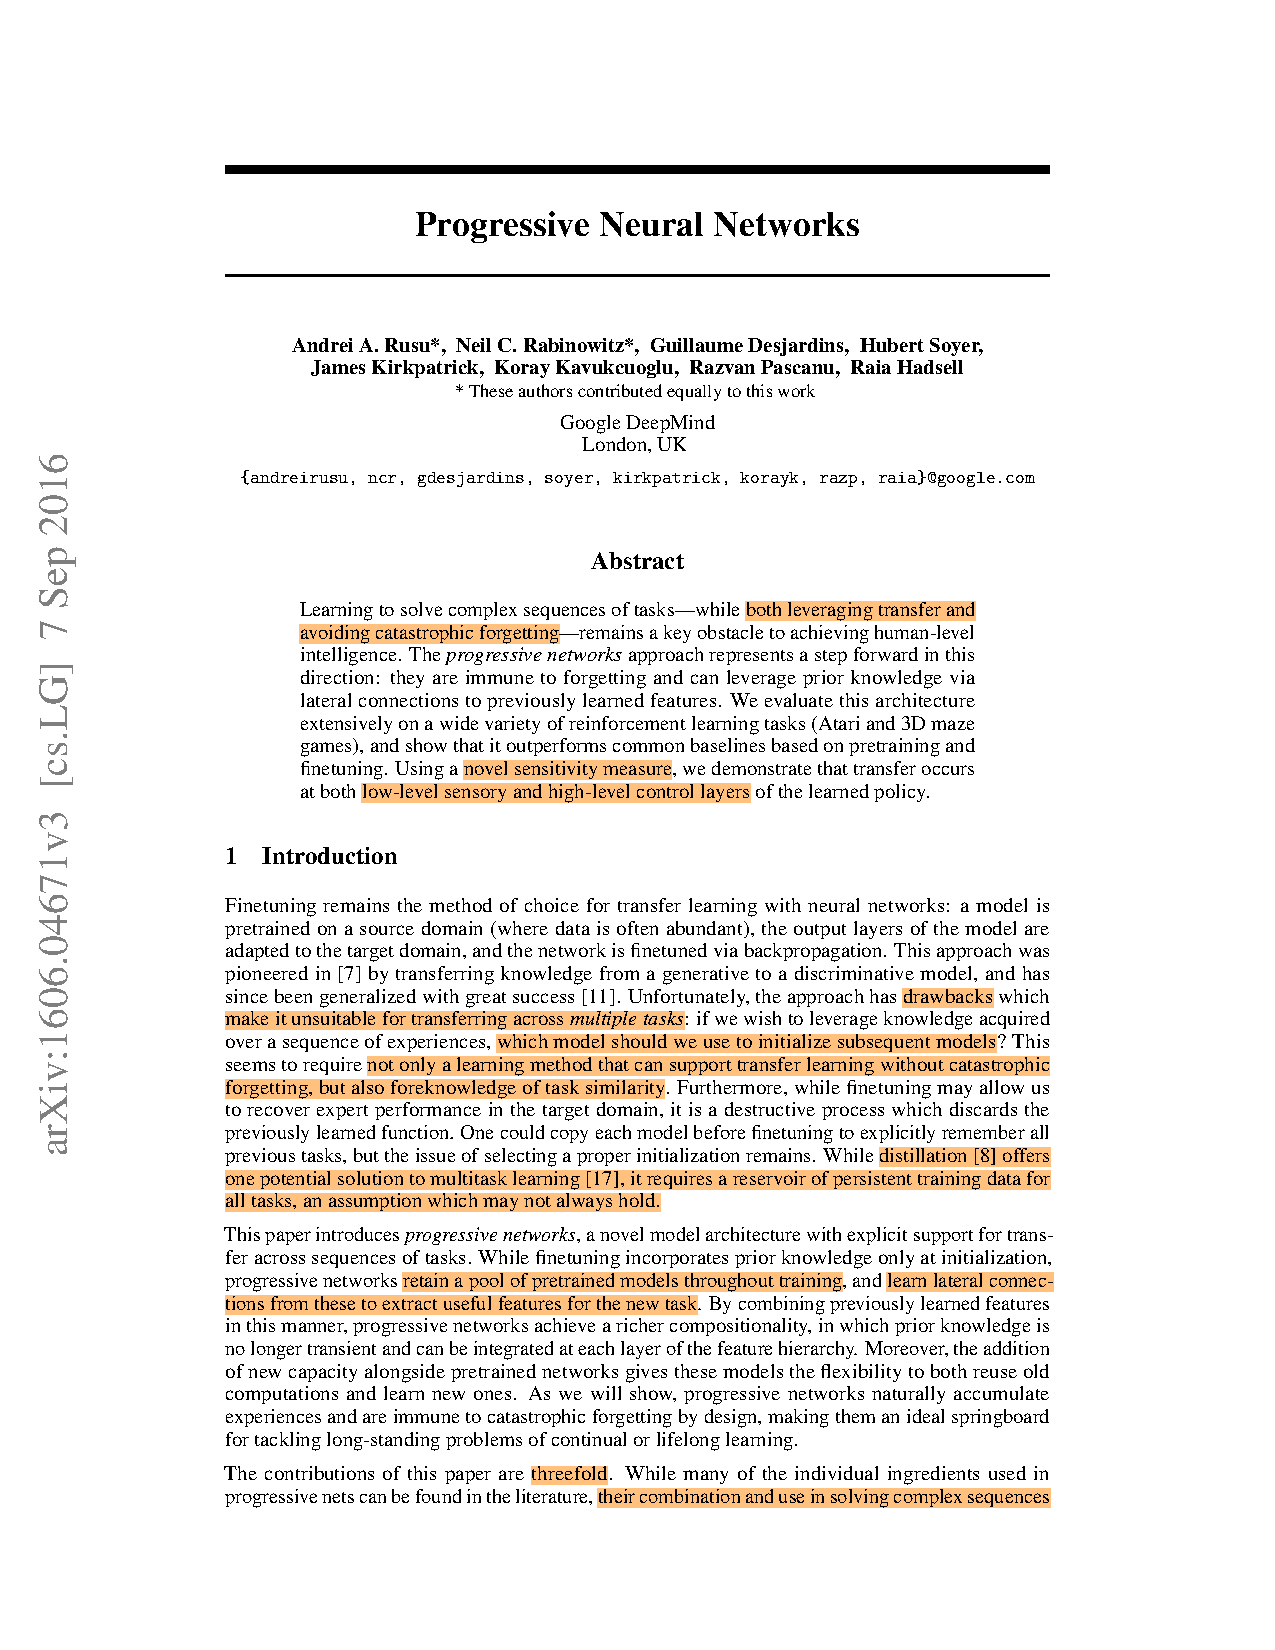
\includegraphics[scale=2]{img/pnn.png}
    %       \caption{An Example of K=3 Progressive Neural Network}
    %       \label{fig:pnn}
    %     \end{figure}
    % \end{block}
    
    \begin{block}{Progressive Neural Networks\cite{rusu2016progressive} (cont'd)}
        Advantage of Progressive Neural Networks
        \begin{itemize}
            \item Catastrophic forgetting is prevented by instantiating a new neural network (a $column$) for each task being solved.
            \item Learning can be accelerated by utilizing learned feature from previous columns via lateral connections.
            \item $K$ independent tasks can be solved at the end of the training.
        \end{itemize}
        \vspace{0.5in}
        \begin{figure}
          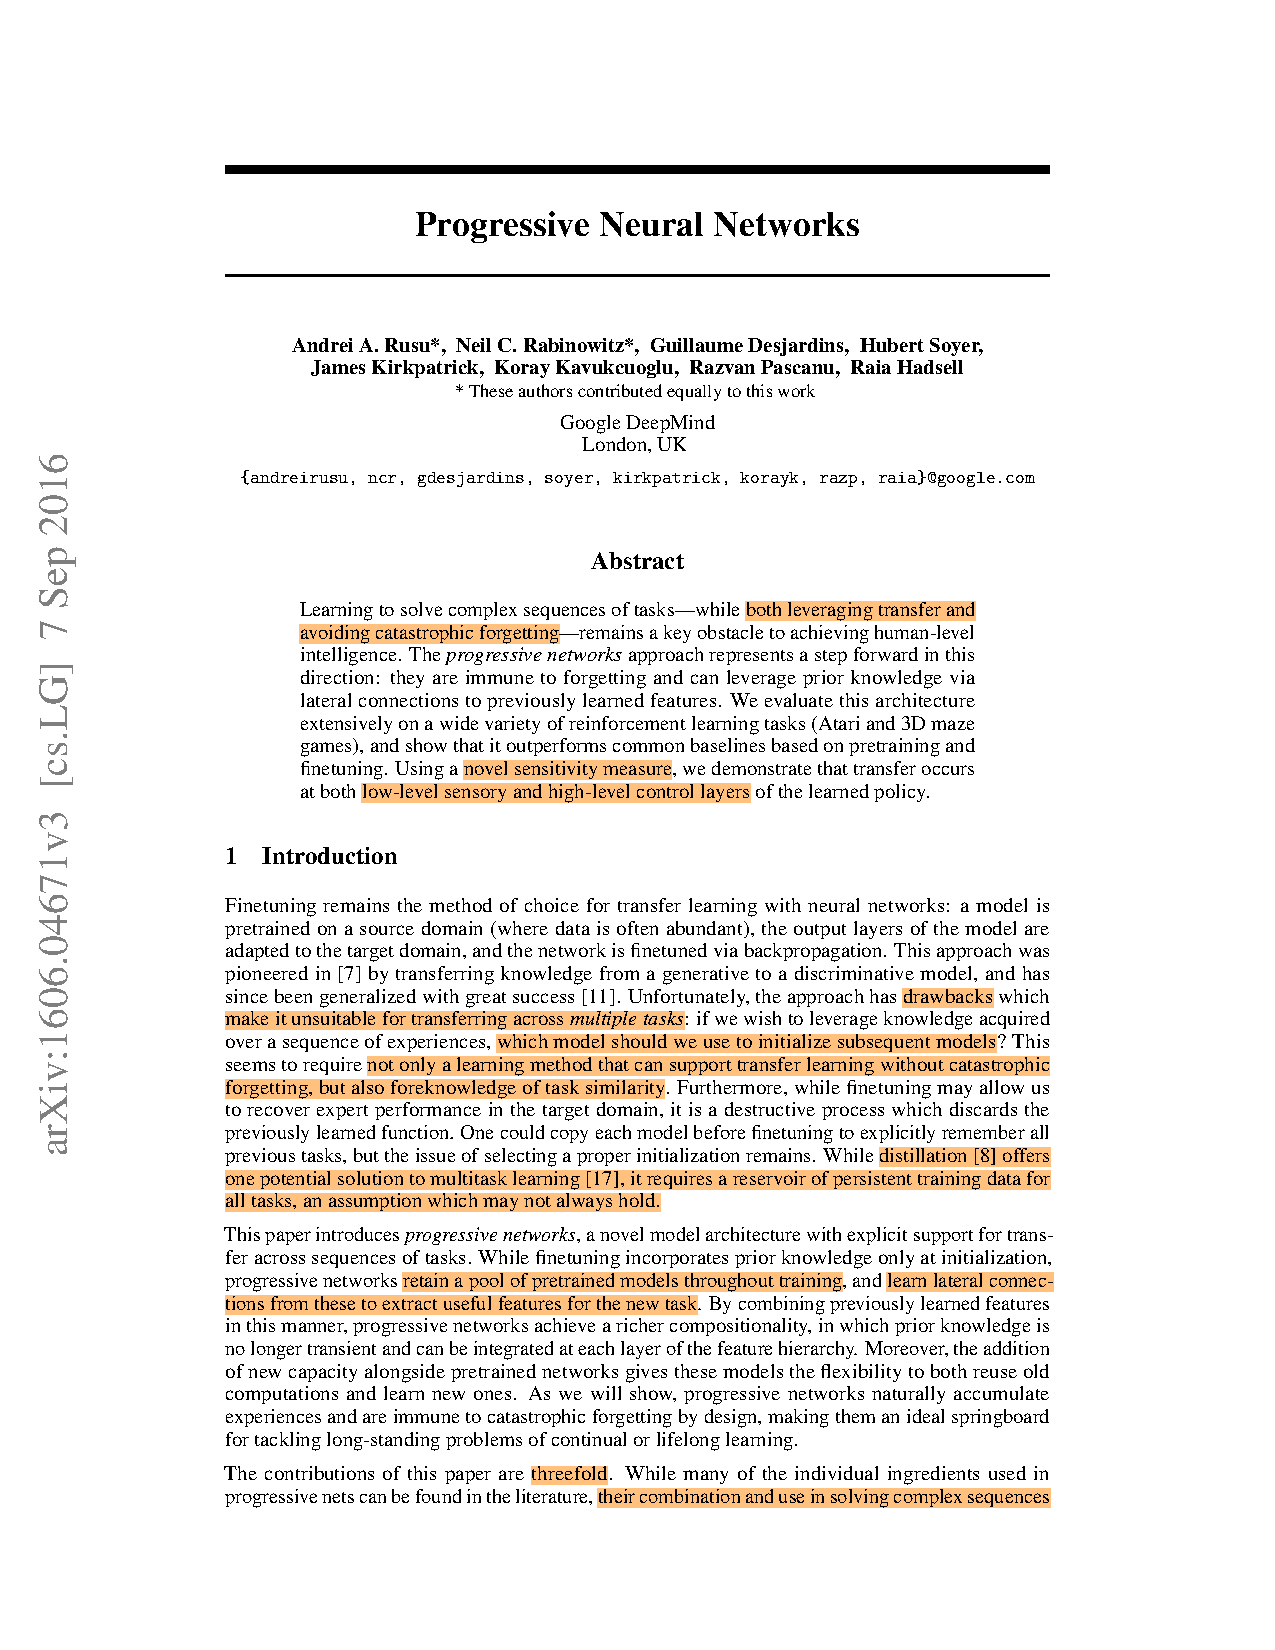
\includegraphics[width=0.4\textwidth]{img/pnn.png}
          \caption{An Example of K=3 Progressive Neural Network}
          \label{fig:pnn}
        \end{figure}
    \end{block}
    
    \begin{block}{Asynchronous Advantage Actor-Critic Method (A3C) \cite{DBLP:journals/corr/MnihBMGLHSK16}}
    Utilizing the Progressive Neural Networks as a function approximator, this paper uses A3C method to update agent policy. Instead of having only one agent interacting with the environment, A3C method emphasizes on creating multiple local agents interacting with different scenarios in the environment, and update the global model asynchronously.
    \begin{figure}
          \includegraphics[width=0.58\textwidth]{img/a3carch.png}
          \caption{A3C}
          \label{fig:A3C}
        \end{figure}
    \end{block}
    \end{column}

    \begin{column}{0.3\linewidth}
    % \begin{block}{Asynchronous Advantage Actor-Critic Method (A3C) (cont'd)}
    %     Updated version of A2C: Same structure but each agent runs A2C locally and updates the global neural network asynchronously.
        
    % \end{block}

    \begin{block}{Result}
        Experiment on Atari game of Pong. The results of training two columns on the Pong variants including:
        \begin{itemize}
            \item $Noisy$ (frozen Gaussian noise is added
to the inputs)
            \item $Black$ (black background)
            \item $White$ (white background)
            \item $Zoom$ (input is scaled by 75%
and translated)
            \item $V-flip$, $H-flip$, $VH-flip$  (input is horizontally and/or vertically flipped)
        \end{itemize}
        \begin{figure}
            \includegraphics[scale=1.4]{img/pongsoupa.png}
            \includegraphics[scale=1.4]{img/pongsoupb.png}
            \caption{(a) Transfer matrix. Colours indicate transfer scores (clipped at 2). For progressive nets, the first column is trained on Pong, Noisy, or H-flip (table rows); the second column is trained on each of the other pong variants (table columns). (b) Example learning curves.}
            \label{fig:eval}
        \end{figure}
    \end{block}

    \begin{block}{References}
        \bibliographystyle{acm}
        {\small \bibliography{ref.bib}}
    \end{block}
    \end{column}

\end{columns}
\end{frame}
\end{document}
